\begin{center}
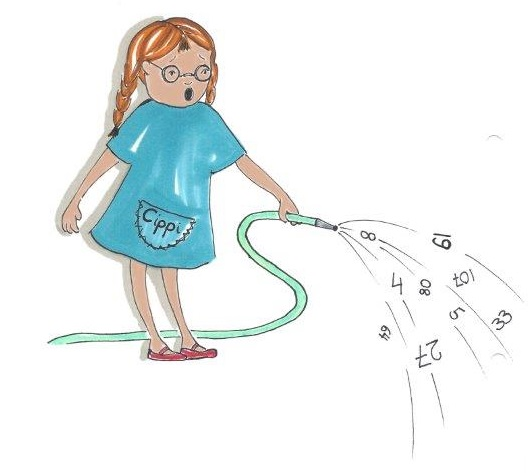
\includegraphics[width=0.6\textwidth]{content/3/chapter6/images/2.png}\\
Cippi waters the flowers
\end{center}

Coroutines are functions that can suspend and resume their execution while keeping their state. The evolution of functions in C++ goes one step further.

\begin{tcolorbox}[colback=red!5!white,colframe=red!75!black,title={The Challenge of Understanding Coroutines}]
	
It was quite a challenge for me to understand coroutines. I strongly suggest that you should not read the sections in the chapter in sequence. Skip in your first iteration the sections “The Framework”, and “The Workflow”. Furthermore, read the case studies “Variations of Futures”, “Modification and Generalization of a Generator”, and “Various Job Workflows”. Reading, studying, and playing with the provided examples should give you an initial intuition need for you to actually dive into details and the workflow of coroutines.
	
\end{tcolorbox}

What I present in this section as a new idea in C++20 is quite old. The term coroutine was coined by \href{https://en.wikipedia.org/wiki/Melvin_Conway}{Melvin Conway}. He used it in his publication on compiler construction in 1963. \href{https://en.wikipedia.org/wiki/Donald_Knuth}{Donald Knuth} called procedures a special case of coroutines. Sometimes, it just takes a while to get your ideas accepted.

\begin{center}
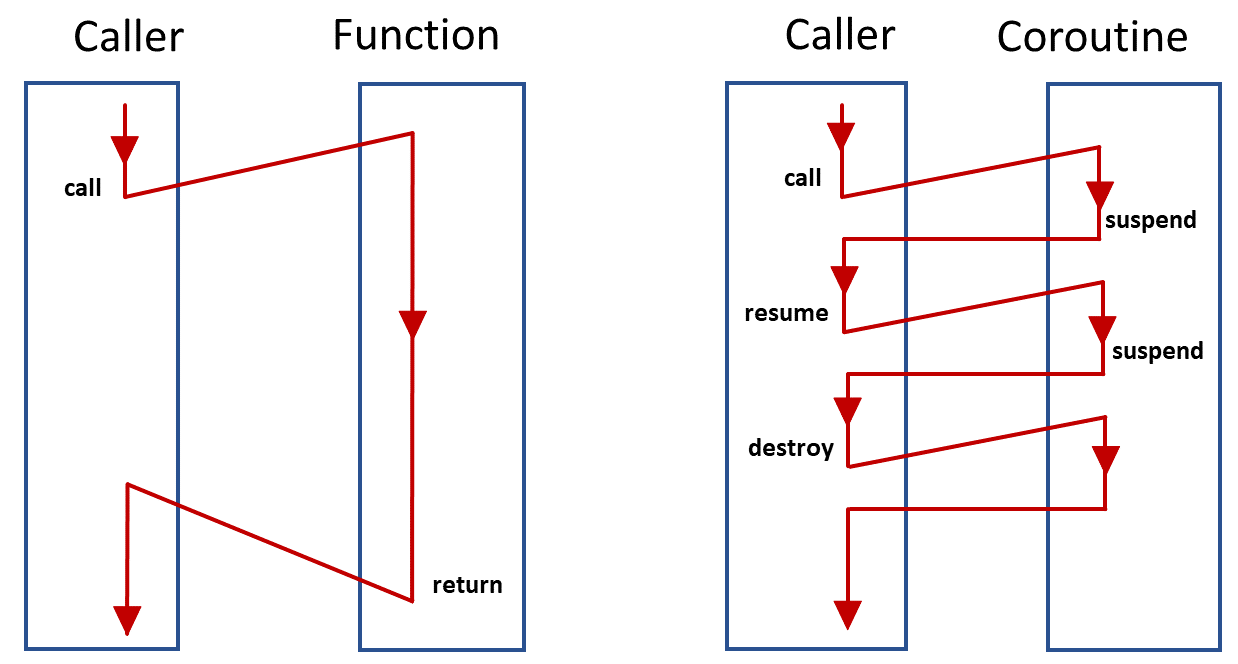
\includegraphics[width=0.6\textwidth]{content/3/chapter6/images/3.png}\\
Functions versus Coroutines
\end{center}

While you can only call a function and return from it, you can call a coroutine, suspend and resume it, and destroy a suspended coroutine.

With the new keywords co\_await and co\_yield, C++20 extends the execution of C++ functions with two new concepts.

Thanks to co\_await expression it is possible to suspend and resume the execution of the expression. If you use co\_await expression in a function func, the call auto getResult = func() does not block if the result of the function is not available. Instead of resource-consuming blocking, you have resource-friendly waiting.

co\_yield expression supports generator functions. The generator function returns a new value each time you call it. A generator function is a kind of data stream from which you can pick values. The data stream can be infinite. Therefore, we are at the center of lazy evaluation with C++.

\subsubsubsection{6.1.1\hspace{0.2cm} A Generator Function}

The following program is as simple as possible. The function getNumbers returns all integers from begin to end, incremented by inc. Value begin has to be smaller than end, and inc has to be positive.

\hspace*{\fill} \\ %插入空行
\noindent
A greedy generator function
\begin{lstlisting}[style=styleCXX]
// greedyGenerator.cpp

#include <iostream>
#include <vector>

std::vector<int> getNumbers(int begin, int end, int inc = 1) {

	std::vector<int> numbers;
	for (int i = begin; i < end; i += inc) {
		numbers.push_back(i);
	}
	
	return numbers;

}

int main() {

	std::cout << '\n';
	
	const auto numbers= getNumbers(-10, 11);
	
	for (auto n: numbers) std::cout << n << " ";
	
	std::cout << "\n\n";
	
	for (auto n: getNumbers(0, 101, 5)) std::cout << n << " ";
	
	std::cout << "\n\n";

}
\end{lstlisting}

Of course, I am reinventing the wheel with getNumbers, because that job could be done with \href{http://en.cppreference.com/w/cpp/algorithm/iota}{std::iota}.

For completeness, here is the output.

\begin{center}
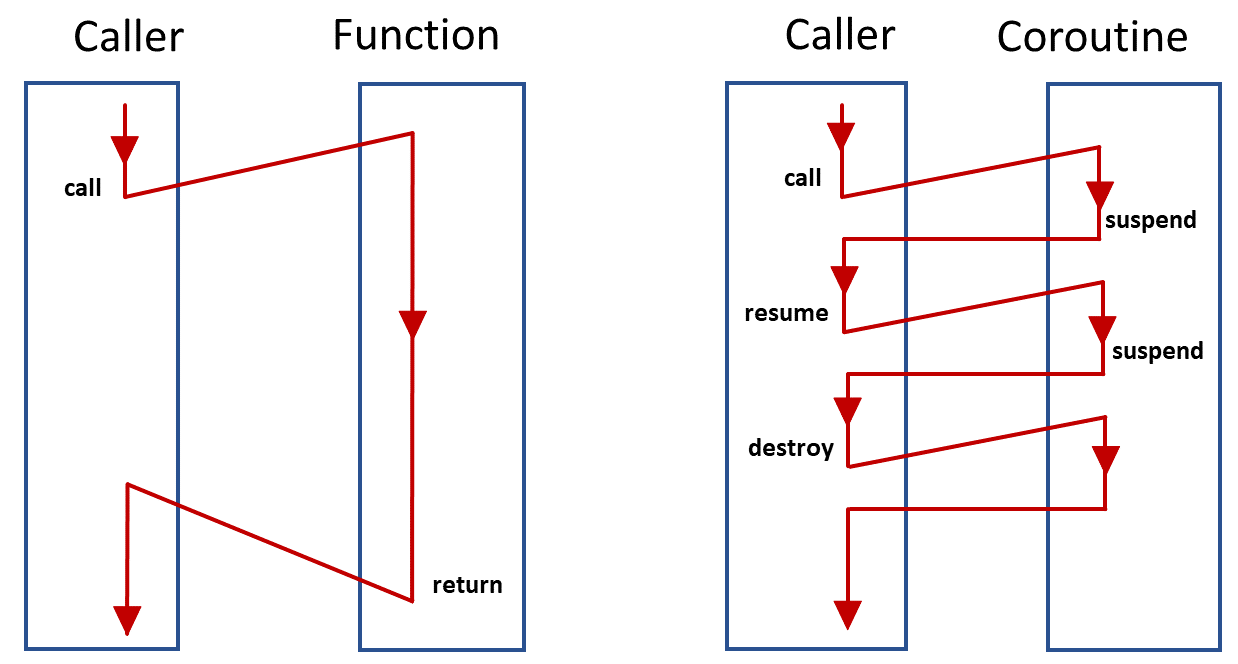
\includegraphics[width=0.4\textwidth]{content/3/chapter6/images/3.png}\\
A generator function
\end{center}

Two observations of the program greedyGenerator.cpp are essential. On the one hand, the vector numbers in line 8 always gets all values. This holds even if I’m only interested in the first 5 elements of a vector with 1000 elements. On the other hand, it’s quite easy to transform the function getNumbers into a lazy generator. The following program is intentionally not complete. The definition of the generator is still missing.

\hspace*{\fill} \\ %插入空行
\noindent
A lazy generator function
\begin{lstlisting}[style=styleCXX]
// lazyGenerator.cpp

#include <iostream>

generator<int> generatorForNumbers(int begin, int inc = 1) {

	for (int i = begin;; i += inc) {
		co_yield i;
	}

}

int main() {

	std::cout << '\n';
	
	const auto numbers = generatorForNumbers(-10);
	
	for (int i= 1; i <= 20; ++i) std::cout << numbers() << " ";
	
	std::cout << "\n\n";
	
	for (auto n: generatorForNumbers(0, 5)) std::cout << n << " ";
	
	std::cout << "\n\n";

}
\end{lstlisting}

While the function getNumbers in the file greedyGenerator.cpp returns a std::vector<int>, the coroutine generatorForNumbers in lazyGenerator.cpp returns a generator. The generator numbers in line 17 or generatorForNumbers(0, 5) in line 23 returns a new number on request. The range-based for loop triggers the query. Precisely, the query of the coroutine returns the value i via co\_yield i and immediately suspends its execution. If a new value is requested, the coroutine resumes its execution exactly at that place.

The expression generatorForNumbers(0, 5) in line 23 is a just-in-place use of a generator. I want to stress one point explicitly. The coroutine generatorForNumbers creates an infinite data stream because the for loop in line 8 has no end condition. This is fine if I only ask for a finite number of values, such as in line 20. This does not hold for line 23, since there is no end condition. Therefore, the expression runs forever.

\subsubsubsection{6.1.2\hspace{0.2cm} Characteristics}

Coroutines have a few unique characteristics.

\hspace*{\fill} \\ %插入空行
\noindent
\textbf{6.1.2.1\hspace{0.2cm} Typical Use Cases}

Coroutines are the usual way to write \href{https://en.wikipedia.org/wiki/Event-driven_programming}{event-driven applications}, which can be simulations, games, servers, user interfaces, or even algorithms. Coroutines are also typically used for \href{https://en.wikipedia.org/wiki/Computer_multitasking}{cooperative multitasking}. The key to cooperative multitasking is that each task takes as much time as it needs, but avoids sleeping or waiting, and instead allows some other task to run. Cooperative multitasking stands in contrast to pre-emptive multitasking, for which we have a scheduler that decides how long each task gets the CPU.

There are different kinds of coroutines.

\hspace*{\fill} \\ %插入空行
\noindent
\textbf{6.1.2.2\hspace{0.2cm} Underlying Concepts}

Coroutines in C++20 are asymmetric, first-class, and stackless.

The workflow of an asymmetric coroutine goes back to the caller. This does not hold for a symmetric coroutine. A symmetric coroutine can delegate its workflow to another coroutine.

First-class coroutines are similar to first-class functions, since coroutines behave like data. Behaving like data means that you can use them as arguments to or return values from functions, or store them in a variable.

A stackless coroutine can suspend and resume the top-level coroutine. The execution of the coroutine and the yielding from the coroutine comes back to the caller. The coroutine stores its state for resumption separate from the stack. Stackless coroutines are often called resumable functions.

\hspace*{\fill} \\ %插入空行
\noindent
\textbf{6.1.2.3\hspace{0.2cm} Design Goals}

Gor Nishanov describes in proposal \href{https://isocpp.org/files/papers/N4402.pdf}{N4402} the design goals of coroutines.

Coroutines should

\begin{itemize}
\item 
be highly scalable (to billions of concurrent coroutines)

\item 
have highly efficient resume and suspend operations comparable in cost to the overhead of a function

\item 
seamlessly interact with existing facilities with no overhead

\item 
have open-ended coroutine machinery allowing library designers to develop coroutine libraries exposing various high-level semantics such as generators, \href{https://tour.golang.org/concurrency/1}{goroutines}, tasks and more

\item 
usable in environments where exceptions are forbidden or not available
\end{itemize}

Due to the design goals of scalability and seamless interaction with existing facilities, the coroutines are stackless. In contrast, a stackful coroutine reserves a default stack of 1MB on Windows, and 2MB on Linux.

There are four ways for a function to become a coroutine.

\hspace*{\fill} \\ %插入空行
\noindent
\textbf{6.1.2.4\hspace{0.2cm} Becoming a Coroutine}

A function becomes a coroutine if it uses

\begin{itemize}
\item 
co\_return, or

\item 
co\_await, or

\item 
co\_yield, or a

\item 
co\_await expression in a range-based for loop.
\end{itemize}

\begin{tcolorbox}[colback=red!5!white,colframe=red!75!black,title={Distinguish Between the Coroutine Factory and the Coroutine Object}]
	
The term coroutine is often used for two different aspects of coroutines: the function invoking co\_return, co\_await, or co\_yield, and the coroutine object. Using one term for two different coroutine aspects may puzzle you (such as it did me). Let me clarify both terms.

\hspace*{\fill} \\ %插入空行
\noindent
A simple coroutine producing 2021
\begin{lstlisting}[style=styleCXX]
MyFuture<int> createFuture() {
	co_return 2021;
}

int main() {
	
	auto fut = createFuture();
	std::cout << "fut.get(): " << fut.get() << '\n';
	
}
\end{lstlisting}

This straightforward example has a function createFuture and returns an object of type MyFuture<int>. Both are called coroutines. To be specific, the function createFuture is a coroutine factory that returns a coroutine object. The coroutine object is a resumable object that implements the framework to model a specific behavior. I present in the section co\_return the implementation and the use of this straightforward coroutine.
	
\end{tcolorbox}

\hspace*{\fill} \\ %插入空行
\noindent
\textbf{6.1.2.4.1 \hspace{0.2cm} Restrictions}

Coroutines cannot have return statements or placeholder return types. This holds for unconstrained placeholders (auto), and constrained placeholders (concepts).

Additionally, functions having \href{https://en.cppreference.com/w/cpp/language/variadic_arguments}{variadic arguments}, constexpr functions, consteval functions, constructors, destructors, and the main function cannot be coroutines.

\subsubsubsection{6.1.3\hspace{0.2cm} The Framework}

The framework for implementing coroutines consists of more than 20 functions, some of which you must implement and some of which you may overwrite. Therefore, you can tailor the coroutine to your needs.

A coroutine is associated with three parts: the promise object, the coroutine handle, and the coroutine frame. The client gets the coroutine handle to interact with the promise object, which keeps its state in the coroutine frame.

\hspace*{\fill} \\ %插入空行
\noindent
\textbf{6.1.3.1\hspace{0.2cm} Promise Object}


\hspace*{\fill} \\ %插入空行
\noindent
\textbf{6.1.3.2\hspace{0.2cm} Coroutine Handle}


\hspace*{\fill} \\ %插入空行
\noindent
\textbf{6.1.3.3\hspace{0.2cm} Coroutine Frame}

\subsubsubsection{6.1.4\hspace{0.2cm} Awaitables and Awaiters}


\hspace*{\fill} \\ %插入空行
\noindent
\textbf{6.1.4.1\hspace{0.2cm} Awaitables}


\hspace*{\fill} \\ %插入空行
\noindent
\textbf{6.1.4.2\hspace{0.2cm} The Concept Awaitable}


\hspace*{\fill} \\ %插入空行
\noindent
\textbf{6.1.4.3\hspace{0.2cm} std::suspend\_always and std::suspend\_never}


\hspace*{\fill} \\ %插入空行
\noindent
\textbf{6.1.4.4\hspace{0.2cm} initial\_suspend}


\hspace*{\fill} \\ %插入空行
\noindent
\textbf{6.1.4.5\hspace{0.2cm} final\_suspend}


\hspace*{\fill} \\ %插入空行
\noindent
\textbf{6.1.4.6\hspace{0.2cm} Awaiter}


\subsubsubsection{6.1.5\hspace{0.2cm} The Workflows}


\hspace*{\fill} \\ %插入空行
\noindent
\textbf{6.1.5.1\hspace{0.2cm} The Promise Workflow}


\hspace*{\fill} \\ %插入空行
\noindent
\textbf{6.1.5.2\hspace{0.2cm} The Awaiter Workflow}



\subsubsubsection{6.1.6\hspace{0.2cm} co\_return}

\hspace*{\fill} \\ %插入空行
\noindent
\textbf{6.1.6.1\hspace{0.2cm} A Future}

\subsubsubsection{6.1.7\hspace{0.2cm} co\_yield}

\hspace*{\fill} \\ %插入空行
\noindent
\textbf{6.1.7.1\hspace{0.2cm} An Infinite Data Stream}

\subsubsubsection{6.1.8\hspace{0.2cm} co\_await}

\hspace*{\fill} \\ %插入空行
\noindent
\textbf{6.1.8.1\hspace{0.2cm} Starting a Job on Request}

\hspace*{\fill} \\ %插入空行
\noindent
\textbf{6.1.8.2\hspace{0.2cm} Thread Synchronization}
